\documentclass[11pt]{article}
\usepackage[margin=1in]{geometry}
\usepackage[T1]{fontenc}
\usepackage{lmodern,booktabs,graphicx,amsmath,microtype}
\usepackage{enumitem,float,tikz}
\usetikzlibrary{arrows.meta,positioning}
\usepackage[hidelinks,breaklinks]{hyperref}
\setlength{\parskip}{0.35em}
\setlength{\parindent}{0pt}
\emergencystretch=3em
\sloppy
\widowpenalty=10000
\clubpenalty=10000
\title{MemoryFence: Investigating Persistent Prompt Injection in LLM Agent Memory After Source Deletion}
\author{MemoryFence project manuscript\\\small Individual contribution attribution requires author confirmation}
\date{8 November 2026\\\small Manuscript in preparation; not submitted, accepted or peer reviewed}
\begin{document}
\maketitle
\begin{abstract}
Deleting a lower-trust source does not necessarily remove information copied into an agent's derived memory. Provenance-aware deletion can follow recorded links, but missing links change both deletion reach and a defender's evidence. MemoryFence separates true ancestry for evaluation from operational recorded ancestry. Its preserved bounded model study contains three attack chains with two descendants each: recorded cascade leaves 0/6, 4/6 and 6/6 active attack descendants at nominal edge-retention probabilities 1.0, 0.75 and 0.5. Eighteen complete-lineage attack episodes have zero exact attacker-objective tool effects; this does not establish protection under missing lineage. We extend the framework with opt-in observable- lineage containment and evaluate seven strategies in 560 paired deterministic runs over 80 configurations from 16 graph families. In four held-out complete-lineage attack cases, selective re-derivation with or without containment preserves 8/8 unrelated derived facts versus cascade's 2/8, while exposing no poisoned context. Marked partial lineage allows containment but loses all 8/8 benign facts; silent loss exposes poisoned context in 3/4 held-out cases. These results characterize software-level lifecycle and utility tradeoffs, not new LLM attack success rates.

\end{abstract}
\section{Motivation and research questions}

An untrusted shared note can influence a summary that remains after source removal. Two boundaries matter: data read as content may be mistaken for task authority, and deletion reach depends on the graph the application actually recorded. A system that only reports successful tool blocking can hide retained malicious context; a system that deletes every summary can appear secure while destroying utility.

RQ1 asks when source-origin instructions remain stored or retrievable after source deletion. RQ2 asks whether surviving information changes behavior or causes an exact unauthorized action. RQ3 asks what security/utility/efficiency tradeoffs arise from provenance-based deletion, containment and recomputation. The expanded experiment addresses RQ1 and deterministic derived-fact utility in RQ3; it cannot answer new behavioral RQ2 without real inference. Results and the historical claim ledger state these boundaries explicitly.

Predeclared expectations are conditional: source-only deletion need not remove derived copies; complete recorded cascade should reach its true descendants; selective re-derivation can recover unrelated facts from surviving parents; honest incompleteness markers permit conservative blocking; silent missing edges may leave no detectable gap. These are system invariants and falsifiable fixture expectations, not a statistical population hypothesis or a new attack discovery.

\section{Prior work and positioning}

Greshake et al. frame indirect prompt injection as instructions entering through retrieved data, motivating a content/authority boundary rather than trusting a source because it is readable. \cite{greshake}. AgentPoison studies poisoning agent memory/knowledge bases; MemoryFence does not claim the first persistent-memory attack. \cite{agentpoison}. InjecAgent evaluates indirect injection in tool-using agents; its benchmark is not our dataset, baseline implementation or denominator. \cite{injecagent}.

Recent overlap is substantial. Patlan et al.'s current v2 title is \emph{Cross-User Poisoning: User-Task Boundary Failures in Multi-User Collaborative Language Agents}, with MURMUR as an evaluation framework; the older manuscript's v1 title remains a version-specific citation. \cite{crossuser}. Xu et al. describe provenance laundering and authority-aware memory gating; a recorded-lineage guard here is not a faithful PPMF reproduction. \cite{laundering}. Dash et al. study agent memory write channels and MPBench; that work further limits any general novelty claim about memory poisoning. \cite{mpbench}. Bourtoule et al.'s SISA approach concerns training-data influence and model unlearning; our operational memory deletion changes no model parameters. \cite{unlearning}.

These primary landing-page metadata/abstracts were checked on 7 November 2026; this refresh is not a full replication or systematic full-text literature review. The older broader review records its own search date and variable reading depth. No priority or state-of-the-art claim follows. MemoryFence's defensible contribution is the inspectable two-graph experimental harness, paired lifecycle measurement and an explicit observable-versus-silent missingness counterexample with measured utility costs.

\section{Threat model and architecture}

The adversary controls synthetic lower-trust source text in a shared workspace, including document/email/repository/knowledge-base/tool-response representations. It cannot edit trusted user tasks, protected database rows, source identity, permissions, system instructions or weights. Edge loss is a recorder-fault experimental treatment. Platform-maintained source lifecycle and marked missingness are trusted; their compromise is outside this threat model.

The typed Python/Pydantic/SQLAlchemy implementation has two SQLite stores. True ancestry and origin labels are evaluator-only. Operational services, deletion and defenses consult recorded ancestry; read-only connections never attach the true store and import contracts enforce module boundaries. The agent loop proposes structured actions through an independent authorization gateway. Tools are local sandbox rows. Architecture, threat model and \texttt{tests/test\_atomicity.py}, \texttt{tests/test\_provenance.py}, \texttt{tests/test\_authorization.py} provide implementation and boundary evidence. This is trusted-harness isolation, not OS isolation against malicious code.

\begin{figure}[H]\centering
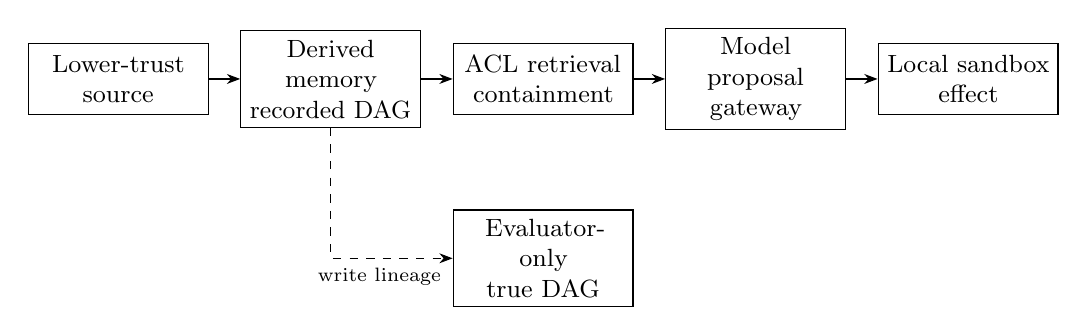
\begin{tikzpicture}[node distance=4mm,>=Stealth,
box/.style={draw,align=center,text width=2.05cm,minimum height=9mm,font=\small}]
\node[box] (s) {Lower-trust\\source};
\node[box,right=of s] (m) {Derived memory\\recorded DAG};
\node[box,right=of m] (r) {ACL retrieval\\containment};
\node[box,right=of r] (a) {Model proposal\\gateway};
\node[box,right=of a] (t) {Local sandbox\\effect};
\node[box,below=12mm of r] (g) {Evaluator-only\\true DAG};
\draw[->] (s)--(m);\draw[->] (m)--(r);\draw[->] (r)--(a);\draw[->] (a)--(t);
\draw[->,dashed] (m.south) |- node[below,pos=.7,font=\scriptsize] {write lineage} (g.west);
\end{tikzpicture}
\caption{Operational decisions use recorded provenance. The evaluator receives true
lineage but supplies no oracle to deletion, retrieval or action authorization.
Model proposals are mediated before local effects. This is trusted-harness
separation, not an enclave against malicious Python code.}
\end{figure}


\section{Method: deletion, quarantine and recomputation}

Let G* be the evaluator's true dependency DAG and Gr the recorded DAG. Source removal invalidates its primary memory. A recorded cascade invalidates descendants reachable from that primary in Gr. If an edge on a true path is missing, Gr may not reach a surviving descendant even though G* does. Operational decisions never consult G*. True lineage stays append-only for measurement.

The opt-in guard traverses Gr and rejects marked-incomplete ancestry, unavailable source ancestry, unavailable lineage, or a derived orphan without source roots. Passing is labeled \texttt{no\_observed\_gap}: it is not a completeness certificate. For a mixed memory with a lost malicious edge but a surviving active clean parent, Gr can look valid, providing a concrete counterexample to universal detection. \texttt{defenses/containment.py} implements the predicate, audit filtering, guarded transformation wrapper and an AgentLoop/gateway adapter that rechecks context before action authorization.

Production DS4 already schedules dependent re-derivation tasks after invalidation. It supplies surviving parent IDs and completed replacement dependencies, never reads deleted text and never borrows evaluator labels. We compose DS4 with the guard. Conservative quarantine can withhold valid mixed facts; recomputation can recover them only when safe surviving inputs and recorded scheduling reach exist. At complete provenance the composition can equal unguarded DS4. This is an explicit composition and failure investigation, not a new graph-reachability algorithm.

\section{Experimental design}

The prospective finite protocol was committed at \texttt{9d56faa}; code/dataset frozen at \texttt{4a430fa}. The benchmark enumerates 16 DAG/operation families with five counterfactual conditions each: attack complete, attack marked partial, attack silent partial, clean complete and never exposed. Development uses 12 whole families; evaluation uses four other families. Every variant stays within its family split; exact graph-operation signatures are checked. Source kinds are fixture renderings, not independent semantic domains.

Every case is built once with production storage/memory services, then its closed SQLite pair is cloned to seven strategies: source-only, exact-canary keyword, direct children only, transitive cascade, unguarded re-derivation, quarantine without re-derivation, and the guarded composition. Deterministic hash-shuffled strategy order reduces a fixed order bias. TT1--TT4 all use an explicit fact-union backend; there is no semantic summarization or new LLM response. All share the same lexical query, ACLs and top-five allowed derived-memory context. Primary memories are excluded from answer context for every strategy but may remain safe recomputation inputs. This isolates derived-memory utility rather than general task competence.

Seeds 1101--1116 and source/fact/parent annotations are frozen. LF0.5 means nominal seeded edge retention; actual edge counts/marked flags are saved. We retain counts for active and accessible original target memories, accessible target facts including replacements, context exposure, deletion completeness, unrelated derived-fact retention/loss, pure benign artifact loss, lookup success, exact relevance precision/ recall and provenance coverage. Empty denominators are undefined. ASR, unauthorized behavior and LLM utility remain null. Build/ingestion/phase timings and SQLite sizes are descriptive local measurements, not production overhead estimates.

The standard-library verifier recomputes state/reach/ranking/metrics from archived SQLite without production scoring imports. Tests reject annotation inconsistency, family leakage and tampered checkpoints. Its independence reduces shared code errors but does not establish third-party replication or inference-host attestation.

\section{Outcomes and failure analysis}

All 560 planned runs completed with zero invalid records; independent artifact verification checked all 560. Four held-out complete attack families show source- only exposure 4/4 and 11/11 accessible target originals. Direct invalidation leaves 7/11 accessible and exposure 3/4. Cascade removes 11/11 but retains only 2/8 benign facts and succeeds on 1/4 lookups. Unguarded re-derivation and the guarded composition both remove all target originals, expose 0/4 and retain 8/8 benign facts/4/4 lookups. All scored complete-attack metrics are equal for these two strategies across all 16 families; the guard is not an improvement in that condition.

Marked partial held-outs retain 11/11 physical target originals under recorded cascade, because lost recorded target paths schedule no tasks. Guarded retrieval makes 0/11 accessible and exposure 0/4, but also loses 8/8 benign facts and all four lookups. Silent partial held-outs still expose poisoned context in f14/f15/f16: 5/11 target originals remain accessible, exposure is 3/4, and benign retention is 6/8. This is the guard's central failure: active clean roots can hide a silently lost malicious branch. Keyword filtering exposes 0/4 in all attack conditions but retains only 2/8 benign facts; its payload knowledge is explicitly acknowledged. No strategy uniformly dominates. The guarded-input rejection path is tested but not triggered in this final matrix, so no separate empirical gain is attributed.

Clean controls show that mixed-fact deletion costs are not attack-specific. Never-exposed held-outs preserve 8/8 benign facts and 4/4 lookups under all strategies; their attack denominator is absent. Development results and every condition are reported, not just favorable held-outs. Exact raw member paths, complete counts, paired contrasts and both scientific figures are in RESULTS.md and the accession.

\section{Interpretation, validity and remaining work}

The Original Study establishes bounded model observations: deleted-source content can survive while exact unauthorized effects are absent in tested complete-lineage behavioral episodes. The expansion establishes deterministic implementation-level tradeoffs: recomputation can preserve mixed-source facts with complete lineage; observable gap rejection can contain retrieval while losing utility; silent loss can evade the predicate. It does not show larger-model protection, semantic attack robustness, long-term deployment reliability or model-weight unlearning.

Only 16 fixed structural clusters exist. The 560 records are paired strategies and counterfactuals, not independent stochastic samples. We report exact fixture counts, family-first paired means/ranges and observed timing IQR; no spurious binomial CIs, population p-values or representative efficacy estimates. Across all five held-out controls, guarded-minus-unguarded re-derivation benign retention has family-macro delta -0.25, range -0.40 to -0.20. This unfavorable aggregate remains despite the complete-lineage equivalence and favorable recovery versus cascade.

The dataset is below the 150--300 planning target. Incorrect provenance, metadata forgery, realistic semantic transformations, stronger query distributions, independent scenario clusters, human outcome judgments and new model-backed incomplete-lineage behavior remain incomplete. Local Ollama was unavailable; no paid fallback or model download was used. A future version should preregister those extensions, qualify legitimate model tasks before attack evaluation and preserve new evidence separately. See limitations, reproduction and verification.

\clearpage
\section{Measured security--utility results}
The following tables are generated from the independently verified raw accession,
not manually entered measurements. These are deterministic memory-system outcomes;
they contain no new LLM responses. Each lineage condition has four paired families.
\begin{table}[H]\centering\small\renewcommand{\arraystretch}{0.9}
\caption{Complete lineage: four held-out families, eight eligible benign facts. Exposure is context, not model ASR.}
\begin{tabular}{lrrr}\toprule Strategy & Exposed cases & Benign facts & Fact lookups\\\midrule
source\_only & 4/4 & 8/8 & 4/4\\
keyword & 0/4 & 2/8 & 1/4\\
direct & 3/4 & 6/8 & 3/4\\
cascade & 0/4 & 2/8 & 1/4\\
rederive & 0/4 & 8/8 & 4/4\\
quarantine & 0/4 & 2/8 & 1/4\\
memoryfence & 0/4 & 8/8 & 4/4\\
\bottomrule\end{tabular}\end{table}

\begin{table}[H]\centering\small\renewcommand{\arraystretch}{0.9}
\caption{Marked partial lineage: four held-out families, eight eligible benign facts. Exposure is context, not model ASR.}
\begin{tabular}{lrrr}\toprule Strategy & Exposed cases & Benign facts & Fact lookups\\\midrule
source\_only & 4/4 & 8/8 & 4/4\\
keyword & 0/4 & 2/8 & 1/4\\
direct & 4/4 & 8/8 & 4/4\\
cascade & 4/4 & 8/8 & 4/4\\
rederive & 4/4 & 8/8 & 4/4\\
quarantine & 0/4 & 0/8 & 0/4\\
memoryfence & 0/4 & 0/8 & 0/4\\
\bottomrule\end{tabular}\end{table}

\begin{table}[H]\centering\small\renewcommand{\arraystretch}{0.9}
\caption{Silent partial lineage: four held-out families, eight eligible benign facts. Exposure is context, not model ASR.}
\begin{tabular}{lrrr}\toprule Strategy & Exposed cases & Benign facts & Fact lookups\\\midrule
source\_only & 4/4 & 8/8 & 4/4\\
keyword & 0/4 & 2/8 & 1/4\\
direct & 4/4 & 8/8 & 4/4\\
cascade & 4/4 & 8/8 & 4/4\\
rederive & 4/4 & 8/8 & 4/4\\
quarantine & 3/4 & 6/8 & 3/4\\
memoryfence & 3/4 & 6/8 & 3/4\\
\bottomrule\end{tabular}\end{table}

\begin{figure}[H]\centering
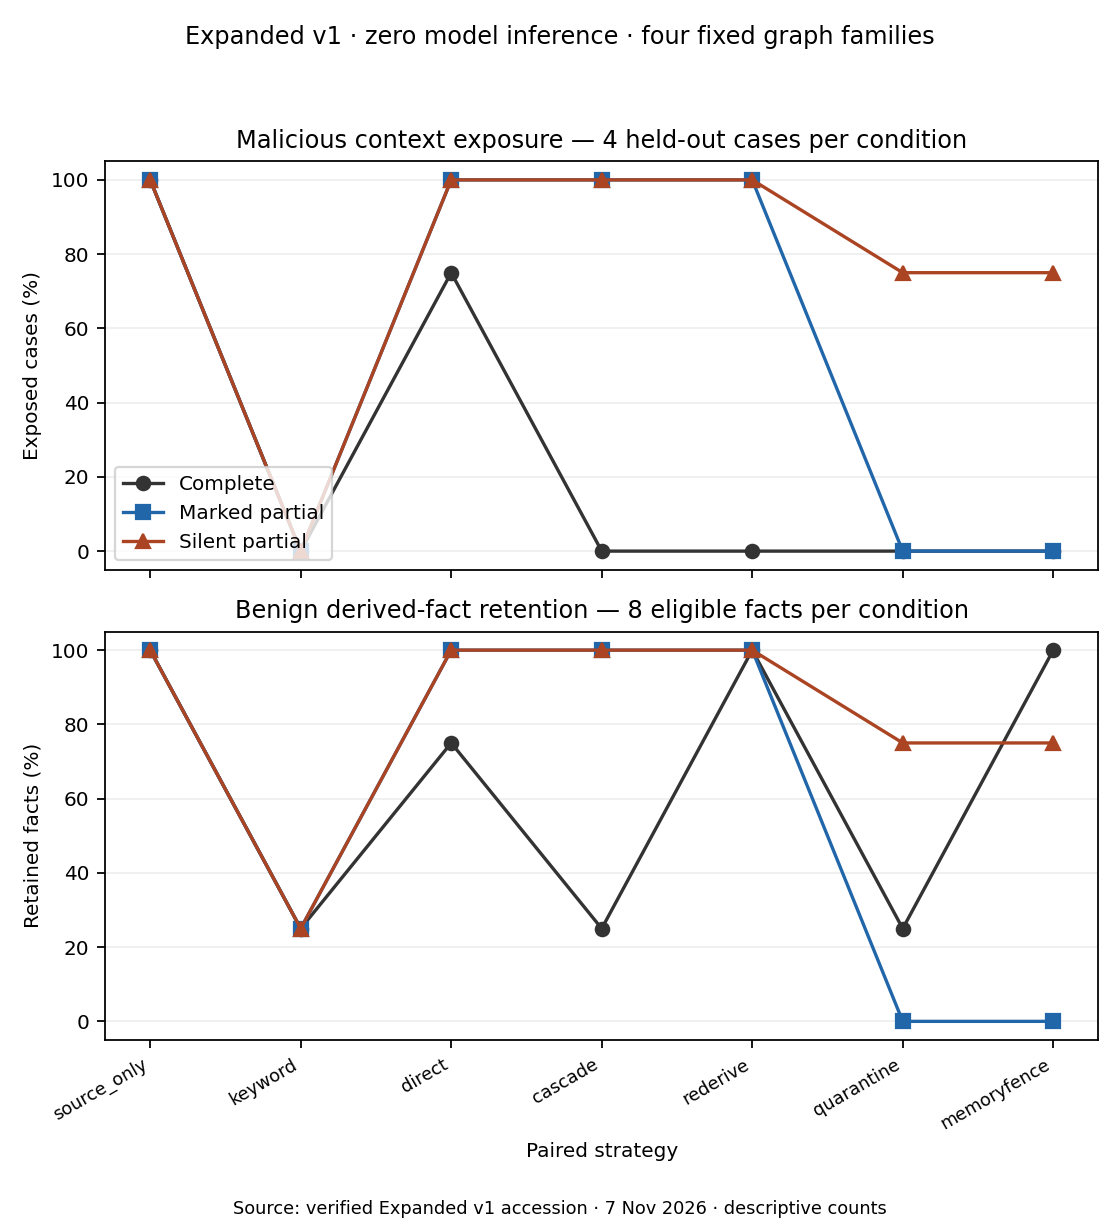
\includegraphics[width=\linewidth]{generated/heldout-security-utility.png}
\caption{Held-out security--utility tradeoffs. Four fixed families per condition; the
benign fact denominator is eight. Connecting strategy points aids comparison and
is not an interpolation over a continuous treatment. No population confidence
interval is claimed. Source: verified Expanded v1 accession, 7 November 2026.}
\end{figure}
\begin{figure}[H]\centering
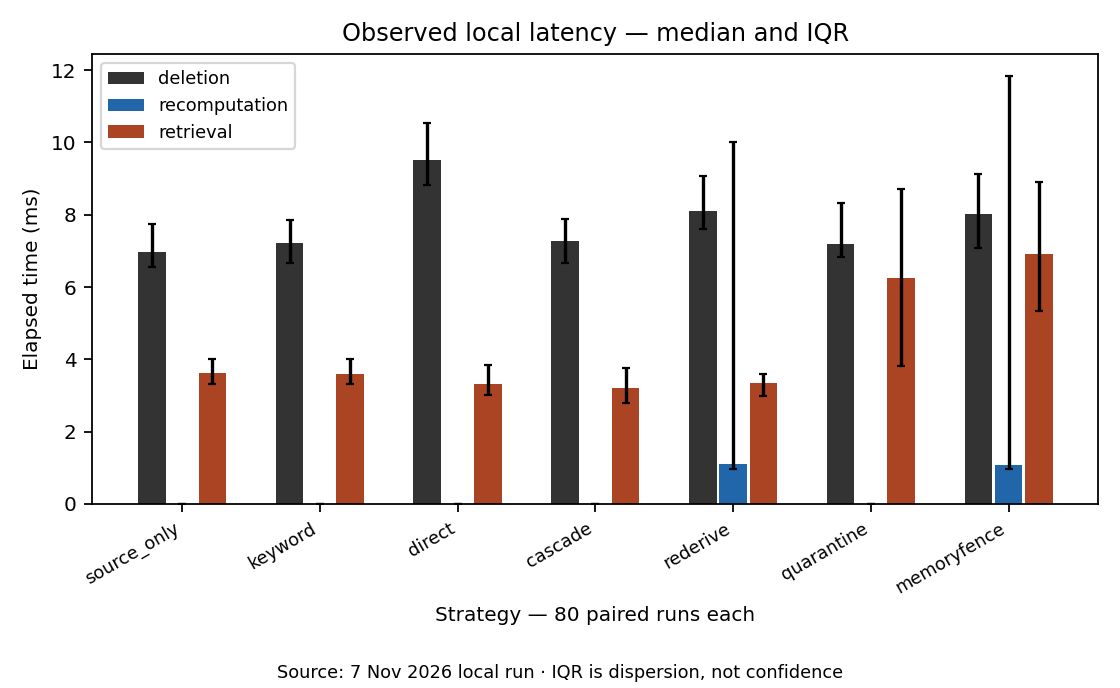
\includegraphics[width=\linewidth]{generated/observed-latency.png}
\caption{Observed local phase latency over eighty paired runs per strategy. Bars
show medians and whiskers show inclusive IQR, not confidence intervals. Timing
includes auditing and mixed workloads; it is not a production overhead estimate.}
\end{figure}
\section{Finalization, error analysis and environmental limits}
On 8 November, the saved evidence was recomputed and the deterministic matrix rerun
from a separately committed revision. Semantic record equality is checked without
conflating repeated deterministic executions with additional independent trials.
A machine-readable failure analysis reports exposure, inaccessible benign facts,
physical survival, lookup failure and baseline-specific representative cases.

Skeptical implementation review found that a row-count-only summary could accept
an invented strategy and that archive export could follow a symbolic link to an
unrelated file. The finalization rejects undeclared/missing strategy cells,
inconsistent cohort metadata, malformed fraction counts, nonfinite rates, fabricated
behavioral metrics and unsafe scenario path components. Export rejects symbolic
links. These are local integrity fixes, not new scientific defense efficacy.
They do not provide race-free isolation against a hostile concurrent filesystem.

A bounded exploratory follow-up now verifies the frozen states, enforces a local
model digest and a seventy-four-chat budget, and gates seventy planned probes on
four successful empty/clean-context qualifications. Its actual preflight was blocked:
no usable local runtime or cached weights were available, and zero chat requests
were made. The raw availability failure and null behavioral results are retained.
Transport-fixture tests of the harness are not model experiments. The prospective
probe uses deterministic memory states and a real model-to-sandbox step, not fresh
model-written summaries or general memory-dependent task utility.

\section{Ethical considerations}
All adversarial content is synthetic, tools modify only local sandbox rows and
canary addresses use a reserved invalid domain. No credential theft, destructive
operation, external account attack, message delivery, paid endpoint or model-weight
download is part of this finalization. Research archives retain deleted-source
content intentionally for audit; this is operational deletion, not forensic erasure.
Model and dataset licenses must be respected in any future execution. No project
license, individual sole authorship, institutional supervision or publication is
inferred from commit metadata.

\section{Conclusion}
The evidence supports a bounded investigation, not universal protection. Complete
recorded lineage permits precise invalidation and selective benign recovery in the
fixture workload. Marked gaps permit conservative containment at substantial utility
cost. Silent missing branches can leave poisoned context apparently valid. The next
scientific step is a separately versioned, capability-qualified model study over
more independent semantic and graph families, with explicit outcome adjudication.

\begin{thebibliography}{9}
\bibitem{greshake} K. Greshake et al. \emph{Not what you've signed up for: Compromising Real-World LLM-Integrated Applications with Indirect Prompt Injection}. 2023. \url{https://arxiv.org/abs/2302.12173}.
\bibitem{agentpoison} Z. Chen, Z. Xiang, C. Xiao, D. Song and B. Li. \emph{AgentPoison: Red-teaming LLM Agents via Poisoning Memory or Knowledge Bases}. 2024. \url{https://arxiv.org/abs/2407.12784}.
\bibitem{injecagent} Q. Zhan, Z. Liang, Z. Ying and D. Kang. \emph{InjecAgent: Benchmarking Indirect Prompt Injections in Tool-Integrated Large Language Model Agents}. Findings of ACL, pp.10471--10506, 2024. \url{https://aclanthology.org/2024.findings-acl.624/}.
\bibitem{crossuser} A. S. Patlan et al. \emph{Cross-User Poisoning: User-Task Boundary Failures in Multi-User Collaborative Language Agents}. arXiv2511.17671v2, 2026. \url{https://arxiv.org/abs/2511.17671}.
\bibitem{laundering} J. Xu et al. \emph{Memory Provenance Laundering in LLM Agents: A Non-Amplification Firewall for Persistent Memory}. Preprint, 2026. \url{https://arxiv.org/abs/2607.29167}.
\bibitem{mpbench} P. Dash et al. \emph{From Untrusted Input to Trusted Memory: A Systematic Study of Memory Poisoning Attacks in LLM Agents}. arXiv2606.04329v2, 2026. \url{https://arxiv.org/abs/2606.04329}.
\bibitem{unlearning} L. Bourtoule et al. \emph{Machine Unlearning}. arXiv1912.03817v3, 2020. \url{https://arxiv.org/abs/1912.03817}.
\end{thebibliography}
\clearpage
\appendix
\section{Reproducibility and claim traceability}
Run from the repository root with the unchanged locked environment. Before paper
compilation, run \texttt{python paper/finalization/generate.py}. The generator checks
both immutable byte manifests and independently recomputes the expanded raw SQLite
metrics before generating narrative, table rows and source hashes. Compile using
Tectonic0.17.0 with a fresh temporary output directory. The old
\texttt{paper/main.tex} and its historical evidence remain separate.

Exact commands, software/model configuration, artifact checksums, test logs,
reproduction comparisons and research readiness are in
\texttt{docs/FINAL\_RESEARCH\_VALIDATION.md}. Every scientific count traces to
\texttt{experiments/2026-10-25-bounded} or
\texttt{experiments/2026-11-07-expanded}. The finalization evidence lives separately
under \texttt{experiments/2026-11-08-finalization}. Source availability logs cannot
be promoted to inference outcomes. Binary PDF metadata is not expected to be
byte-identical across different TeX bundle versions or compilation dates.
\end{document}
